\documentclass[notitlepage,a4paper,10pt,normalheadings]{article}

% \usepackage{mathpazo} 
\usepackage{ngerman} 
\usepackage[latin1]{inputenc} 
\usepackage[T1]{fontenc} 
\usepackage[pdftex]{graphicx} 
\usepackage[pdftex,bookmarks=true,colorlinks,linkcolor=blue,urlcolor=blue,citecolor=blue]{hyperref}

\sloppy

%opening
\title{Mozilla Thunderbird\\installieren und nutzen}
\author{German Privacy Foundation e.V.}
\date{\today}

\hypersetup {
    pdftitle= { Mozilla Thunderbird installieren und nutzen }
    pdfkeywords= {Mozilla Thunderbird }
}


\begin{document}
\maketitle
\tableofcontents
\section{E-Mail Provider}
Als erstes braucht man eine oder mehrere E-Mail Adressen. Es ist empfehlenswert, f�r unter�schiedliche Anwendungen auch verschiedene E-Mail Adressen zu verwenden. Es erschwert die Profilbildung anhand der E-Mail Adresse und verringert die Spam-Bel�stigung. Wenn Amazon, Ebay oder andere kommerzielle Anbieter zu aufdringlich werden, wird die mit Spam �ber�schwemmte E-Mail Adresse einfach gel�scht ohne die private Kommunikation zu st�ren.\\

Neben einer sehr privaten E-Mail Adresse f�r Freunde k�nnte man weitere E-Mail Adressen f�r Eink�ufe im Internet nutzen oder f�r politische Aktivit�ten. Um nicht st�ndig viele E-Mail Accounts abfragen zu m�ssen, kann man die f�r Eink�ufe im Internet genutzt E-Mail Accounts auch an die private Hauptadresse weiterleiten lassen. Alle Mail-Provider bieten diese Option. Bei den gro�en deutschen Mail Providern GMX.de und WEB.de gibt es bis zu 100 Fun-Domains extra f�r diesen Zweck. Bereits mit der kostenlosen Version kann man bis zu 3 Fun-Adressen nutzen.\\ 

Wenn eine E-Mail Adresse nur f�r die Anmeldung in einem Forum oder das Ver�ffentlichen eines Kommentars in Blogs ben�tigt wird, kann man \textit{tempor�re Mailadressen} nutzen (siehe weiter unten).\\

Eine kleine Liste von E-Mail Providern abseits des Mainstream:
\begin{itemize}
 \item \textbf{Posteo.de} \footnote{ \href{https://posteo.de/}{https://posteo.de}} und \textbf{aikQ.de} \footnote{ \href{https://www.aikq.de/}{https://www.aikq.de}} (deutsche Mailprovider, Accounts ab 1,- Euro pro Monat, anonyme Accounts m�glich mit Bezahlung per Brief)
 \item \textbf{VFEmail} \footnote{ \href{https://www.vfemail.net/}{https://www.vfemail.net}} (anonymer Mailprovider, ben�tigt eine Wegwerf-Adresse f�r Registrierung, kostenfreie Accounts mit POP3/SMTP und beliebig vielen tempor�ren E-Mail Adressen)
 \item \textbf{CryptoHeaven} \footnote{ \href{https://www.cryptoheaven.com/index.shtml}{https://www.cryptoheaven.com/}} (Accounts ab \$60 pro Jahr, einfache Verschl�sselung der Kommunikation mit Accounts beim gleichen Provider, Offshore registrierte Firma, Server in Kanada)
 \item \textbf{XMAIL.net} \footnote{ \href{https://www.xmail.net}{https://www.xmail.net}} (die Betreiberfirma Aaex Corp. ist auf den British Virgin Islands registriert, die Server stehen in Kanada, kostenfrei Accounts mit POP3, aber ohne SMTP)
 \item \textbf{runbox.com} \footnote{ \href{https://secure.runbox.com/}{https://secure.runbox.com/}} (norwegischer E-Mail Provider, Server stehen ebenfalls in Norwegen, Accounts ab 1,66 Dollar pro Monat)
 \item \textbf{neomailbox.com} \footnote{ \href{http://www.neomailbox.com/services/secure-email}{http://www.neomailbox.com/services/secure-email}} (anonymes E-Mail Hosting in der Schweiz, Accounts ab 3,33 Dollar pro Monat, anonyme Bezahlung mit Pecunix oder Liberty Reserve m�glich)
\end{itemize}

F�r politische Aktivisten gibt es Anbieter, die insbesondere den Schutz vor staatlichem Zugriff hervorheben. Diese Anbieter werden mit Spenden finanziert. F�r einen Account muss man seine politischen Aktivit�ten nachweisen, aber nicht unbedingt seine Identit�t offen legen. Neben E-Mail Accounts werden auch Blogs und Mailinglisten angeboten.
\begin{itemize}
 \item \textbf{Associazione-Investici} \footnote{ \href{http://www.autistici.org/de/get\_service.html}{http://www.autistici.org/de/get\_service.html}} (italienischer Provider, Server stehen bei XS4ALL in Niederlande, verwendet eigene Certification Authority f�r SSL-Zertifikate)
 \item \textbf{Nadir.org} \footnote{ \href{http://www.nadir.org/}{http://www.nadir.org}} (deutscher Provider, Server stehen ebenfalls bei XS4ALL)
 \item \textbf{AktiviX.org} \footnote{ \href{https://www.aktivix.org/}{https://www.aktivix.org}} (deutscher Provider, Server stehen in Brasilien)
\end{itemize}

Hinweis: es kostet Geld, einen zuverl�ssigen Mailservice bereitzustellen. Es ist durchaus sinnvoll, die \textit{alles kostenlos Mentalit�t} f�r einen vertrauensw�rdigen Mailprovider fallen zu lassen.

\subsubsection*{Webinterfaces der Mail-Provider sind oft unsicher}
Die Webinterfaces der Mail-Provider bieten �berwiegend eine unsichere Konfiguration der HTTPS-Verschl�sselung des Webinterface. Oft ist es f�r einen Angreifer m�glich, eine schwache, abh�rbare Verschl�sselung zu erzwingen. Insecure Renegotiation wird teilweise noch verwendet oder das veraltete SSLv2 wird noch unterst�tzt. Das Problem betrifft nicht nur die Webseiten der Mail-Provider. Nach einer Studie bieten nur 10\% der Websites sichere Verschl�sselung nach dem Stand der Technik.\footnote{ \href{http://www.heise.de/developer/meldung/SSL-Pulse-protokolliert-Sicherheit-von-Webseiten-1569214.html}{http://www.heise.de/developer/meldung/SSL-Pulse-protokolliert-Sicherheit-von-Webseiten-1569214.html}}\\

Die folgenden Provider wurden mit dem \textit{SSL-Test von Qualys SSL Labs}\footnote{ \href{https://www.ssllabs.com/ssltest/index.html}{https://www.ssllabs.com/ssltest}} �berpr�ft: 
\begin{itemize}
 \item Posteo: sichere HTTPS-Verschl�sselung
 \item aikQ: sichere HTTPS-Verschl�sselung
 \item neomailbox.com: sichere HTTPS-Verschl�sselung
 \item VFEmail: sichere HTTPS-Verschl�sselung mit aktuellen Browsern
 \item CryptoHeaven: schwache Verschl�sselung und SSLv2 unterst�tzt
 \item XMAIL.net: schwache Verschl�sselung und SSLv2 werden unterst�tzt
 \item Runbox.com Insecure Renegotiation, SSLv2 wird unterst�tzt
\end{itemize}
 
Aus diesem Grund sollte man einen E-Mail Client nutzen. Die Verschl�sselung f�r POP3 und SMTP ist bei den oben genannten Providern auf dem aktuellen Stand der Technik. Da viele E-Mail Provider POP3 und SMTP nur f�r Premium-Kunden anbieten, sollte man nicht an der falschen Stelle sparen und sich nicht mit einem kostenfreien Account via Webinterface begn�gen. 

\subsubsection*{Nicht empfohlene E-Mail Provider}
Einige Gr�nde, warum verschiedene E-Mail Provider mit gutem Ruf nicht in die Liste der Empfehlungen aufgenommen wurden:
\begin{itemize}
 \item Hushmail speichert zuviel Daten. Neben den �blichen Daten beim Besuch der Webseite werden die E-Mails gescannt und folgende Daten unbegrenzt lange gespeichert:
\begin{enumerate}
 \item alle Sender- und Empf�nger E-Mail Adressen (VDS-artig)
 \item alle Dateinamen der empfangenen und gesendeten Attachements
 \item Betreffzeilen aller E-Mails (nicht verschl�sselbar)
 \item URLs aus dem Text unverschl�sselter E-Mails
 \item ... and any other information that we deem necessary
\end{enumerate}
Diese Daten werden bei der K�ndigung eines Account NICHT gel�scht.\\

Bei der Bezahlung f�r einen Premium-Account werden die IP-Adresse des Kunden sowie Land, Stadt und PLZ an Dritte weitergeben. Au�erdem bindet Hushmail.com Dienste von Drittseiten ein. Die ID des Hushmail Account wird beim Besuch der Webseite nach dem Login an diese Drittseiten �bermittelt. F�r die Privacy-Policy dieser Drittseiten �bernimmt Hushmail.com keine Verantwortung.
\item In der EU-Studie \textit{Fighting cyber crime and protecting privacy in the cloud}\footnote{ \href{http://www.europarl.europa.eu/committees/en/studiesdownload.html?languageDocument=EN\&file=79050}{http://www.europarl.europa.eu/committees/en/studiesdownload.html?languageDocument=EN\&file=79050}} warnen die Autoren in Kapitel 5.4 (S. 48) vor Risiken bei der Speicherung von Daten in den USA. Aufgrund des \textit{US PATRIOT Act} (insbesondere S. 215ff) und der \textit{4. Erg�nzung des FISA Amendments Act} ist es f�r US-Beh�rden ohne juristische Kontrolle m�glich, die Kommunikation von Nicht-US-B�rgern zu beschn�ffeln. Dabei ist es unerheblich, ob der Cloud- bzw. E-Mail Provider eine US-Firma ist oder nicht. Es reicht nach Ansicht der Amerikaner, wenn die Server in den USA stehen.\\

Aus diesem Grund ist ein Server-Standort \textit{USA} f�r deutsche Nutzer eher ungeeignet. Das betrifft u.a. die E-Mail Provider SecureNym, S-Mail, Fastmail.fm, Lavabit, Rise-up.net...
\item Cotse, Yahoo! und AOL bietet keine sichere Verschl�sselung f�r die Kommunikation zwischen Mail-Server und E-Mail Client (Secure Renegotiation wird nicht f�r SMTP unterst�tzt, was seit seit 2009 als schwerer Fehler im SSL Protokoll eingestuft wird).
\item Weitere Beispiele werden auf der Webseite des Handbuches genannt.\footnote{ \href{https://www.awxcnx.de/handbuch\_31.htm}{https://www.awxcnx.de/handbuch\_31.htm}}
\end{itemize}

\newpage
\section{Mozilla Thunderbird}
Informationen und Downloadm�glichkeiten f�r Mozilla Thunderbird stehen auf der deutschsprachigen Website des Projektes \footnote{ \href{http://www.mozilla.org/de/thunderbird/}{http://www.mozilla.org/de/thunderbird/}} f�r Windows, Linux und MacOS zur Verf�gung.\\

Linux Distributionen enthalten in der Regel Thunderbird. Mit der Paketverwaltung kann Thunderbird und die deutsche Lokalisierung komfortabel installiert und aktualisiert werden. Debian GNU/Linux bietet eine angepasste Version von Thunderbird unter dem Namen \textit{Icedove} (allerdings meist in einer veralteten Version). Das Mozilla Debian Team stellt eine aktuellere Version in einem separatem Repository und eine Anleitung\footnote{ \href{http://mozilla.debian.net/}{http://mozilla.debian.net/}} zur Installation bereit.\\

\subsection{Account erstellen}
Nach dem ersten Start von Thunderbird f�hrt ein Assistent durch die Schritte zur Einrichtung eines E-Mail Kontos. Nach Eingabe der E-Mail-Adresse sowie des Passwortes erkennt der Assistent die n�tigen Einstellungen f�r den Mailserver oft automatisch. Es k�nnen auch die Einstellungen eines bisher verwendeten Programms �bernommen werden. Bei der Einrichtung des E-Mail Account sollten einige Punkte beachtet werden.\\

Die Grafik im Bild \ref{abb:email_web} zeigt den Weg einer E-Mail vom Sender zum Empf�nger. In der Regel ist man nicht direkt mit dem Internet verbunden. Der Zugang erfolgt �ber ein Gateway des Providers oder der Firma.\\

\begin{figure}[htb]
\begin{center}
 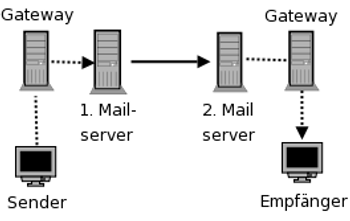
\includegraphics[scale=0.5]{../grafiken/email_weg.png}
\caption{Der Weg einer E-Mail durch das Web}
\label{abb:email_web}
\end{center}
\end{figure}

Der 1. Mailserver nimmt die E-Mail via SMTP entgegen und sendet sie an den 2. Mailserver. Hier liegt die E-Mail, bis der Empf�nger sie abruft und l�scht. Die gestrichelten Verbindungen zu den Mailservern k�nnen mit SSL bzw. TLS kryptografisch gesichert werden. Das hat nichts mit einer Verschl�sselung des Inhalts der E-Mail zu tun. Es wird nur die Daten�bertragung zum Mailserver verschl�sselt und es wird sichergestellt, dass man wirklich mit dem gew�nschten Server verbunden ist. Aktuelle Versionen von Thunderbird aktivieren dieses Feature beim Einrichten eines Account standardm��ig. \\

Wie einfach es ist, unverschl�sselte Verbindungen zu belauschen, die Passw�rter zu extrahieren und das Mail-Konto zu kompromittieren, wurde von T. Pritlove auf der re:publica 2007 demonstriert \footnote{ \href{http://tim.geekheim.de/2007/04/24/netzwerksicherheit-auf-der-republica/}{http://tim.geekheim.de/2007/04/24/netzwerksicherheit-auf-der-republica/}}.\\

Bewusst oder unbewusst k�nnen auch Provider die sichere �bertragung deaktivieren und damit den Traffic mitlesen. Es wird einfach die Meldung des Mail-Servers 250-STARTTLS gefiltert und �berschrieben. Scheinbar verf�gen alle DSL-Provider �ber die M�glichkeit, dieses Feature bei Bedarf f�r einzelne Nutzer zu aktivieren\footnote{ \href{http://heise.de/-206233}{http://heise.de/-206233}}. Die Standard-Einstellung der meisten E-Mail Clients ist \textit{``TLS verwenden wenn m�glich''}. Diese Einstellung ist genau in dem Moment wirkungslos, wenn man es braucht, weil der Traffic beschn�ffelt werden soll.\\

Alle brauchbaren Mail-Server bieten M�glichkeit der verschl�sselten Kommunikation via SSL/TLS oder STARTTLS. Diese Option ist in Thunderbird bei der Einrichtung eines neuen Kontos zu aktivieren. Der Assistent erledigt das in der Regel automatisch.\\

\begin{figure}[htb]
\begin{center}
 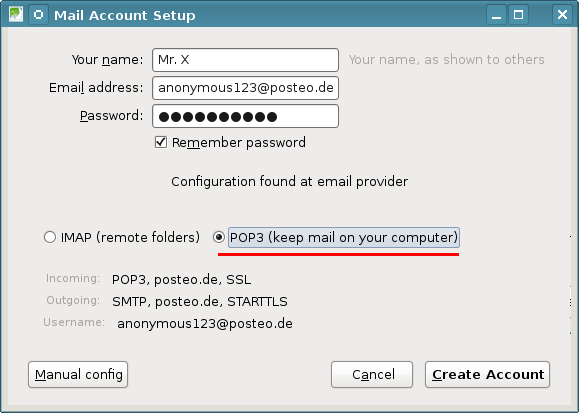
\includegraphics[scale=0.75]{../screenshots/thunderbird_account.png}
\caption{POP3-Account anlegen}
\label{abb:tbaccount1}
\end{center}
\end{figure}

SMTP, POP3 und IMAP sind f�r den Laien verwirrende Abk�rzungen.
\begin{description}
 \item[SMTP] ist das Protokoll zum Versenden von E-Mails.
 \item[POP3] ist das Protokoll zum Herunterladen von empfangenen E-Mails auf den lokalen Rechner. Dabei werden die E-Mails auf dem Server gel�scht.
 \item[IMAP] ist ein Kommunikationsprotokoll, um die empfangenen E-Mails auf dem Server zu verwalten und nur zum Lesen tempor�r herunter zu laden. Auch die versendeten E-Mails werden bei der Nutzung von IMAP auf dem Mailserver des Providers gespeichert.\\

 IMAP bietet damit die M�glichkeit, mit verschiedenen E-Mail Clients von unterschiedlichen Rechnern und Smartphones auf den Account zuzugreifen und stets Zugriff auf alle E-Mails zu haben. Die M�glichkeit des weltweiten Zugriffs auf seine Mails erkauft man sich aber mit Einschr�nkungen des Datenschutzes.\\

 Die auf dem Server des Providers gespeicherten E-Mails unterliegen NICHT mehr dem Tele�kommunikationsgeheimnis nach Artikel 10 GG, wenn der Nutzer Gelegenheit hatte, sie zu l�schen. Das BVerfG hat diese Rechtsauffassung 2009 in dem Urteil 2 BvR 902/06 best�tigt \footnote{ \href{https://www.bundesverfassungsgericht.de/pressemitteilungen/bvg09-079.html}{https://www.bundesverfassungsgericht.de/pressemitteilungen/bvg09-079.html}}.\\

 Mit der Reform der Telekommunikations�berwachung im Dezember 2012 k�nnen Geheim�dienste und Strafverfolge das Passwort f�r den Zugriff auf den Mail-Account ohne richter�liche Pr�fung vom Mail-Provider verlangen und damit Zugang zu dem Postfach erhalten. Es w�re unsch�n, wenn Sie dort die Kommunikation der letzten 5 Jahre vorfinden.
 \end{description}

Deshalb empfehle ich die Nutzung von POP3 (SSL) statt IMAP (Bild \ref{abb:tbaccount1}).\\

F�r viele E-Mail Provoder werden automatisch sichere Einstellungen vom Assistenten vorgeschlagen (SSL bzw. STARTTLS). Wenn keine Vorschl�ge gefunden werden k�nnen, kann man auf \textit{manuelle Konfiguration} klicken und in dem Dialog Bild \ref{abb:tbaccount2} die Einstellungen per Hand anpassen. Die n�tigen Daten f�r POP3- und SMTP-Server findet amn auf der Webseite des Mail-Providers. Au�erdem muss man in der Regel den Usernamen an die Vorgaben des Providers anpassen.
\begin{itemize}
 \item F�r den POP3-Server ist in der Regel Port \textit{995} (SSL) passend.
 \item Viele SMTP-Server bieten neben STARTTLS f�r Port \textit{25} auch auf den Ports \textit{587} (STARTTLS) oder Port \textit{465} (SSL) verschl�sselte Verbindungen zum Senden von E-Mails.
\end{itemize}

\begin{figure}[htb]
\begin{center}
 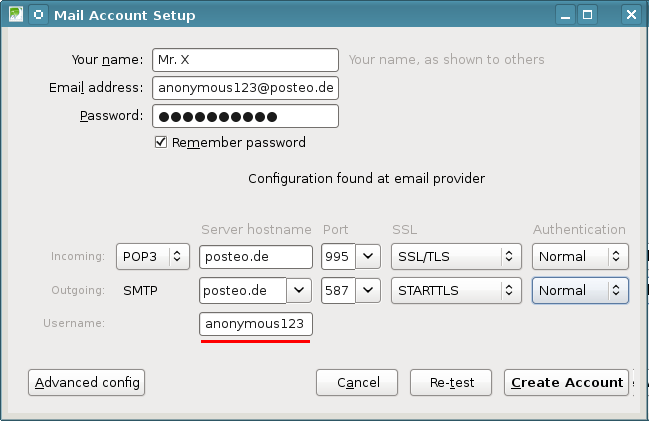
\includegraphics[scale=0.75]{../screenshots/thunderbird_account2.png}
\caption{POP3-Account anpassen}
\label{abb:tbaccount2}
\end{center}
\end{figure}

\subsection{Unsichere Verschl�sselungen deaktivieren}
Aus Gr�nden der Kompatibilt�t mit einigen Mail-Providern unterst�tzt Thunderbird noch immer veraltete und unsichere Verschl�sselungsoptionen f�r die Verbindung zu dem Mailservern. In den \textit{Erweiterten Einstellungen} kann man diese Optionen deaktivieren:
\begin{verbatim}
    security.enable_ssl3                             =  false
    security.ssl.require_safe_negotiation            =  true
    security.ssl.treat_unsafe_negotiation_as_broken  =  true
    security.warn_submit_insecure                    =  true
\end{verbatim} 
Wenn man die im Bild \ref{abb:thunderbird_tlserr} gezeigte, schwer verst�ndliche Fehlermeldung beim Abrufen oder Senden von E-Mails erh�lt, gibt es Probleme beim Aufbau einer sicheren Verbindung und man wechselt am besten den Mail-Provider. Meistens bietet der Server keine Secure Renegotiation beim Aufbau der verschl�sselten Verbindung. Das Problem wird seit 2009 als schwiegend eingestuft \footnote{ \href{https://www.verbraucher-sicher-online.de/news/fehlerhaftes-design-im-wichtigsten-verschluesselungsprotokoll-fuer-angriffe-nutzbar}{https://www.verbraucher-sicher-online.de/news/fehlerhaftes-design-im-wichtigsten-verschluesselungsprotokoll-fuer-angriffe-nutzbar}}.\\

\begin{figure}[htb]
\begin{center}
 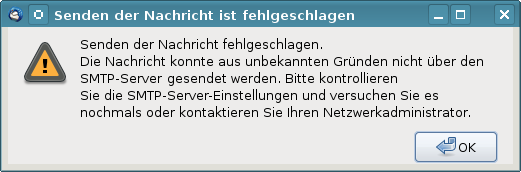
\includegraphics[scale=0.75]{../screenshots/tls-error.png}
\caption{Fehlermeldung bei unsicherer Verbindung}
\label{abb:thunderbird_tlserr}
\end{center}
\end{figure}

In diesem Zusammenhang verweise ich auf die Antwort der Bundesregierung auf eine Kleine Anfrage zu Fernmeldeaufkl�rung des BND vom Mai 2012:
\begin{quote}
  Frage: \textit{Ist die eingesetzte Technik auch in der Lage, verschl�sselte Kommunikation (etwa per SSH oder PGP) zumindest teilweise zu entschl�sseln und/oder auszuwerten?}
\end{quote} 
\begin{quote}
 Antwort: \textit{Ja, die eingesetzte Technik ist grunds�tzlich hierzu in der Lage, \textbf{je nach Art und Qualit�t der Verschl�sselun}g.}
\end{quote} 
Tools zum Ausnutzen der Insecure Renegotiation gibt es auch als OpenSource (z.B. dsniff).

\subsection{Sichere Konfiguration des E-Mail Client}
Einige Hinweise f�r die sichere und unbeobachtete Nutzung des Mediums E-Mail mit Mozilla Thunderbird:
\begin{itemize}
 \item Mit der Verwendung von HTML in E-Mails steht dem Absender ein ganzes Bestiarium von M�glichkeiten zur Beobachtung des Nutzers zur Verf�gung: HTML-Wanzen, Java Applets, JavaScript, Cookies usw. Am einfachsten deaktiviert man diese Features, wenn man nur die Anzeige von \textit{Reinem Text} zul��t. Die Option findet man im Men�punkt \textit{Ansicht -> Nachrichtentext} (siehe Bild \ref{abb:thunderbird_rein_text}). \\

\begin{figure}[htb]
\begin{center}
 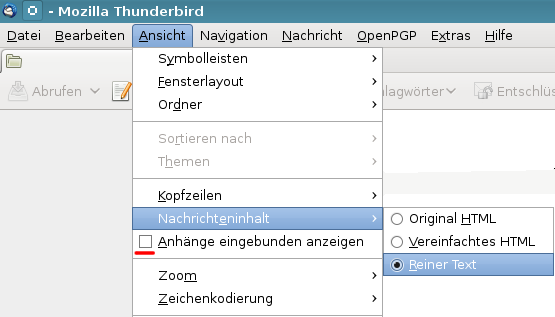
\includegraphics[scale=0.75]{../screenshots/thunderbird_rein.png}
\caption{E-Mails als reinen Text darstellen}
\label{abb:thunderbird_rein_text}
\end{center}
\end{figure}

\item Die Option \textit{Anh�nge eingebunden anzeigen} im Men� \textit{Ansicht} sollte man ebenfalls deaktivieren, um gef�hrliche Anh�nge nicht schon beim Lesen einer E-Mail automatisch zu �ffnen. Der alte Trick mit einem Virus in der E-Mail wird noch immer genutzt, insbesondere wenn man ein Opfer gezielt angreifen will, um den Rechner mit einem Trojaner zu infizieren.

\item Es ist nicht immer m�glich, E-Mails als Plain Text zu lesen. Viele Newsletter sind nur als HTML-Mail lesbar, eBay verwendet ausschlie�lich HTML-Mails f�r Benachrichtigungen usw. In der Regel enthalten diese HTML-only Mails mehrere Trackingelemente.\\

Um diese E-Mails trotzdem lesen zu k�nnen (wenn auch nicht in voller Sch�nheit), kann man die Darstellung \textit{Vereinfachtes HTML} nutzen. Au�erdem k�nnen folgende Features in den \textit{Erweiterten Einstellungen} deaktiviert werden, die jedoch nur f�r die Darstellung von \textit{Orginal HTML} relevant sind: 
\begin{verbatim}
    javascript.enabled                    =  false
    network.cookie.cookieBehavior         =  2
    dom.storage.enabled                   =  false
    geo.enabled                           =  false
    webgl.disabled                        =  true
    layout.css.visited_links_enabled      =  false
    gfx.downloadable_fonts.enabled        =  false
    network.http.sendRefererHeader        =  0
    security.enable_tls_session_tickets   =  false
    network.http.use-cache                =  false
\end{verbatim} 

Alle Bilder in HTML-Mails, die von einem externen Server geladen werden, k�nnen direkt mit der E-Mail Adresse des Empf�ngers verkn�pft sein. Anhand der Logdaten kann der Absender erkennen, wann und wo die E-Mail gelesen wurde. Einige Newsletter verwenden auch HTML-Wanzen. Im Newsletter von Paysafecard findet man beispielsweise ganz unten eine kleine 1x1-Pixel Wanze, die offenbar mit einer individuellen, nutzerspezifischen URL von einem Trackingservice geladen wird: 
\begin{verbatim}
   <IMG src="http://links.mkt3907.com/open/log/43.../1/0">
\end{verbatim} 

Easyjet.com (ein Billigflieger) kann offenbar die Aufrufe seiner Newsletter selbst z�hlen und auswerten. In den E-Mails mit Informationen zu gebuchten Fl�gen findet man folgende kleine Wanze am Ende der Mail:
\begin{verbatim}
   <IMG src="http://mail.easyjet.com/log/bEAS001/mH9..."
        height=0 width=0 border=0>
\end{verbatim}


Um Tracking mit Bildern und HTML-Wanzen zu verhindern, kann man in den \textit{Erweiterten Einstellungen} das Laden externer Bilder blockieren: 
\begin{verbatim}
   permissions.default.image  =  2
\end{verbatim} 

Auch andere Medienformate k�nnen von einem externen Server geladen und als Wanzen genutzt werden. Einen deartigen Einsatz von Audio- oder Videodateien habe ich bisher nicht gefunden, aber technisch w�re es m�glich. Man kann das Laden von Videos und Audiodateien mit folgenden Parametern unterbinden:
\begin{verbatim}
   media.webm.enabled  =  false
   media.wave.enabled  =  false
   media.ogg.enabled   =  false
\end{verbatim} 

Die Links in HTML-Mails f�hren oft nicht direkt zum Ziel sondern werden ebenfalls �ber einen Trackingservice geleitet, der jeden Aufruf des Link individuell f�r jede Empf�nger�adresse protokollieren kann. Als Bespiel soll ein Link aus dem Paysafe�card Newsletter dienen, der zu einem Gewinnspiel bei Paysafecard f�hren soll: 
\begin{verbatim}
   <a href="http://links.mkt3907.com/ctt?kn=28&ms=3N...">
   Gewinne Preise im Wert von 10.000 Euro</a>
\end{verbatim} 

Diesem Tracking kann man nur entgehen, wenn man diese Links in HTML-Mails nicht aufzuruft! Der Trackingservice hat die M�glichkeit, Logdaten von verschiedenen E-Mails zu verkn�pfen und evtl. auch das Surfverhalten einzubeziehen. Wichtige Informationen findet man auch auf der Webseite des Absenders.

\item Die \textit{extension blocklist} kann Mozilla nutzen, um einzelne Add-ons in Thunderbird zu deaktivieren. Es ist praktisch ein kill switch f�r Thunderbird Add-ons. Beim Aktualisieren der Blockliste werden au�erdem detaillierte Informationen an Mozilla �bertragen.\\

Ich mag es nicht, wenn jemand irgendetwas remote auf meinem Rechner deaktiviert oder deaktivieren k�nnte. In den \textit{Erweiterten Einstellungen} kann man das Feature abschalten:
\begin{verbatim}
    extensions.blocklist.enabled = false
\end{verbatim}

\item Gespeicherte Passw�rter f�r den Zugriff auf SMTP-, POP- oder IMAP-Server k�nnen mit einem Masterpasswort gesch�tzt werden.
\end{itemize}


\subsection{Datenverluste vermeiden}
Die folgenden Hinweise wurden von den Mozilla-Entwicklern erarbeitet, um den Nutzer bestm�glich vor Datenverlusten zu sch�tzen:
\begin{itemize}
\item Das Antiviren-Programm ist so einzustellen, dass es den Profilordner von Thunderbird NICHT(!) scannt. Die automatische Beseitigung von Viren kann zu Datenverlusten f�hren.
\item Der Ordner \textit{Posteingang} sollte so leer wie m�glich gehalten werden. Gelesene E-Mails sollten auf themenspezifische Unterordner verteilt werden.
\item Die Ordner sollten regelm��ig komprimiert werden. Hierzu ist mit der rechten Maustaste auf den Ordner zu klicken und der Punkt \textit{Komprimieren} zu w�hlen. W�hrend des Komprimierens sollten keine anderen Aktionen in Thunderbird ausgef�hrt werden.\\

Alternativ kann man in den Einstellungen von Thunderbird in der Sektion \textit{Erweitert} auch eine automatische Komprimierung konfigurieren, sobald es lohnenswert ist (siehe Bild \ref{abb:thunderbird_kompri}). Bei jedem Start pr�ft Thunderbird, ob die Ordner komprimiert werden k�nnen.
\item Regelm��ig sollten Backups des gesamten Profils von Thunderbird angelegt werden. Unter WINDOWS sichert man \textit{C:/Dokumente und Einstellungen/<NAME>/Anwendungsdaten/Thunderbird}, unter Linux ist \textit{\$HOME/.thunderbird} zu sichern.
\end{itemize}

\begin{figure}[htb]
\begin{center}
 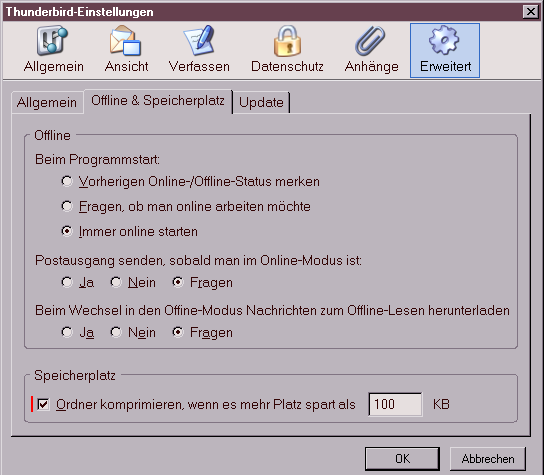
\includegraphics[scale=0.5]{../screenshots/thunderbird_kompri.png}
\caption{Ordner automatisch komprimieren}
\label{abb:thunderbird_kompri}
\end{center}
\end{figure}

\subsection{W�rterb�cher installieren}
Nach der Installation von Thunderbird sind keine W�rterb�cher f�r die Rechtschreibkontrolle vorhanden. Die W�rterb�cher m�ssen zus�tzlich installiert werden, wenn man auf das Feature nicht verzichten m�chte. Nach dem Download der W�rterb�cher \footnote{ \href{https://addons.mozilla.org/de/thunderbird/language-tools/}{https://addons.mozilla.org/de/thunderbird/language-tools/}} ist Thunderbird als zu starten. Der Men�punkt \textit{Extras -> Add-ons} �ffnet den Dialog f�r die Verwaltung. Wenn man oben rechts auf das kleine Werkzeug�symbol klickt (Bild \ref{abb:tbaddons}, kann man die Dateien mit den W�rterb�chern als Add-on installieren.\\

\begin{figure}[htb]
\begin{center}
 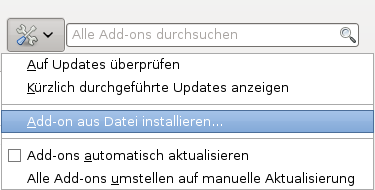
\includegraphics[scale=0.7]{../screenshots/tb-addon-install.png}
\caption{W�rterb�cher in der Add-on Verwaltung installieren}
\label{abb:tbaddons}
\end{center}
\end{figure}

Danach kann man in den Einstellungen von Thunderbird die Rechtschreibpr�fung aktivieren und die bevorzugte Sprache ausw�hlen. Die Auswahl der Sprache kann man beim Schreiben einer Mail jederzeit �ndern. 

\subsection{X-Mailer Kennung modifizieren}
Ich habe gelesen, dass es b�se Buben geben soll, die via Internet ihre Software auf fremden Rechnern installieren m�chten. In diesem Zusammenhang werden oft die Stichworte ``Spambot'' oder ``Bundstrojaner'' genannt.\\

Voraussetzung ist die Kenntnis der vom Opfer genutzten Software. Genau wie jeder Webbrowser sendet auch Thunderbird eine User-Agent-Kennung im Header jeder E-Mail, die Auskunft �ber die genutzte Programmversion und das Betriebssystem liefert. Das folgende (veraltete) Beispiel stammt aus der Mail eines Unbekannten:

\begin{verbatim}
...
User-Agent: Thunderbird 2.0.0.6 (X11/20070728)
X-Enigmail-Version: 0.95.3
...

------- BEGIN PGP MESSAGE -------
Version: GnuPG v1.4.6 (GNU/Linux)
...
\end{verbatim} 

Aha, er nutzt also Thunderbird in der Version 2.0.0.6 unter Linux, hat die Enigmail-Erweiterung v.0.95.3 installiert und verwendet die GnuPG-Version 1.4.6. Das war damals eine typische Kombination f�r Ubuntu Edgy.\\

Die User-Agent-Kennung kann in den erweiterten Einstellungen modifiziert werden. Im Einstellungs-Dialog findet man in der Sektion \textit{Erweitert} den Reiter \textit{Allgemein}. Ein Klick auf den Button Konfiguration bearbeiten �ffnet eine Liste aller Optionen.\\

\begin{figure}[htb]
\begin{center}
 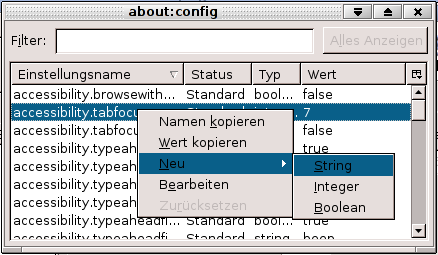
\includegraphics[scale=0.65]{../screenshots/thunderbird_uafake.png}
\caption{Neue Config-Variable anlegen}
\label{abb:thunderbird_uafake}
\end{center}
\end{figure}

Hier f�gt man die neue String-Variable \textbf{general.useragent.override} als neuen Wert ein, indem man mit der rechten Maustaste auf einen freien Bereich klickt und im Kontext-Men� den Punkt \textit{Neu - String} w�hlt.Als Wert f�r diese Variable wird eine leere Zeichenkette eingesetzt. Damit sendet Thunderbird keine Kennung mehr. Nachteile sind nicht erkennbar.\\

Wer das Add-on Enigmail f�r die Verschl�sselung nutzt, sollte dem Add-on die Geschw�tzigkeit abgew�hnen und die Ausgabe von Versionen im Header deaktivieren. Anderenfalls kann ein Schn�ffler anhand einer signierten oder verschl�sselten E-Mail Schlussfolgerungen �ber die verwendete Software ableiten. Folgende Parameter sind in den erweiterten Einstellungen zu setzen:

\begin{verbatim}
   extensions.enigmail.addHeaders            =  false
   extensions.enigmail.useDefaultComment     =  true
   extensions.enigmail.agentAdditionalParam  =  --no-emit-version
\end{verbatim} 

\subsection{Spam-Filter aktivieren}
Das Mozilla Team bezeichnet nicht erw�nschte E-Mails (Spam) als Junk\textit{}. Den integrierten lernf�higen Filter aktiviert man �ber den Men�punkt \textit{Extras -> Junk-Filter}.\\

Im Einstellungsdialog des Filters sollte man die beiden Optionen f�r das automatische Verschieben der Junk-Mails in einen speziellen Ordner aktivieren, am einfachsten in den Ordner \textit{Junk} des entsprechenden Kontos. Au�erdem sollte der lernf�hige Filter aktiviert werden. Ich bin immer wieder von der guten Erkennungsrate beeindruckt.

\subsection{Spam vermeiden}
Man muss nicht bei jeder Gelegenheit im Web seine richtige E-Mail Adresse angeben. Damit f�ngt man sich eine Menge Spam (Junk) ein.\\

Au�erdem ist die E-Mail Adresse ein wichtiges Identit�tsmerkmal. Datensammler verwenden sie als ein Hauptmerkmal f�r die Identifikation, um darauf aufbauend Profile zu erstellen. Stichproben im Internet-Traffic weisen einen hohen Anteil von Suchanfragen nach Informationen zu den Inhabern von E-Mail Adressen aus.\\

Um die eigene E-Mail Adresse nicht zu kompromittieren und trotzdem Angebote zu nutzen, welche die Angabe einer Mailadresse erfordern, kann man tempor�re \textit{Wegwerf-Adressen} nutzen.\\

Bei der Nutzung tempor�rer Mailadressen geht es nicht(!) um die Umgehung der Vorratsdatenspeicherung. Hinweise daf�r findet man im Abschnitt \textit{``E-Mail anonym nutzen''}. Au�erdem ist von einer VDS-artige Speicherung der IP-Adressen auszugehen, wenn der Anbieter keine Angaben zum Datenschutz macht.

\subsubsection*{AnonBox des CCC}
Bei der AnonBox.net des CCC  \footnote{ \href{https://anonbox.net}{https://anonbox.net}} kann ein E-Mail Account f�r den Empfang von einer Nachricht erstellt werden. Der Account ist bis 24:00 Uhr des folgenden Tages g�ltig und nicht verl�ngerbar. Eingehende Nachrichten kann man nur im Webinterface lesen und sie werden nach dem Abrufen gel�scht. Sie k�nnen nur 1x gelesen werden! Zusammen mit der E-Mail wird auch der Account gel�scht. Man kann praktisch nur eine Mail empfangen.\\

Beim Erzeugen einer E-Mail Adresse erh�lt man einen Link, unter dem man ankommende Mails lesen kann. Wenn noch nichts angekommen ist, dann bleibt die Seite leer. Der Link ist als Lese�zeichen zu speichern, wenn man sp�ter nochmal nachschauen m�chte.\\

Die AnonBox bietet als einziger Anbieter SSL-Verschl�sselung und verwendet ein Zertifikat, das von CAcert.org signiert wurde. In den meisten Browsern ist diese CA nicht als vertrauensw�rdig enthalten. Das Root-Zertifikat dieser CA muss von der Webseite zus�tzlich importiert werden. 


\subsubsection*{Wegwerf-Adressen}
Einige Anbieter von Wegwerf-E-Mail-Adressen bieten einen sehr einfach nutzbaren Service, der keinerlei Anmeldung erfordert und auch kein Erstellen der Adresse vor der Nutzung. E-Mail Adressen der Form \textit{pittiplatsch@trash-mail.com} oder \textit{pittiplatsch@weg-werf-email.de} kann man �berall und ohne Vorbereitung unbek�mmert angeben. Das Postfach ist unbegrenzt g�ltig.\\

In einem Webformular auf der Seite des Betreibers findet man sp�ter alle eingegangenen Spam- und sonstigen Nachrichten f�r das gew�hlte Pseudonym. F�r das Webinterface des Postfachs gibt es in der Regel keinen Zugriffsschutz. Jeder, der das Pseudonym kennt, kann die Nachrichten lesen und l�schen. Nachrichten werden nach 6-12h automatisch gel�scht. \\

Liste einiger Anbieter (unvollst�ndig):
\begin{itemize}
 \item \href{http://www.spambog.com/}{http://www.spambog.com} (weitere E-Mail Domains auf der Webseite, Account kann mit Passwort gesichert werden, L�schen der Mails ist m�glich, Session-Cookies erforderlich)
 \item \href{http://onewaymail.com/}{http://onewaymail.com} (weitere E-Mail Domains auf der Webseite, keine Cookies oder Javascript n�tig, E-Mails k�nnen gel�scht werden)
\item \href{http://www.trash-mail.com}{http://www.trash-mail.com} (keine Cookies oder Javascript n�tig, E-Mails k�nnen gel�scht werden)
\item \href{http://www.mailcatch.com/}{http://www.mailcatch.com} (keine Cookies oder Javascript n�tig, E-Mails k�nnen gel�scht werden)
\item \href{http://www.mailinator.com/}{http://www.mailinator.com/} (bietet 5 weitere Domains, keine Cookies oder Javascript n�tig, E-Mails k�nnen gel�scht werden, POP3-Abruf m�glich)
\item \href{http://www.weg-werf-email.de/}{http://www.weg-werf-email.de} (Session-Cookies erforderlich, Passwortschutz m�glich)
\item \href{https://www.guerrillamail.com/}{https://www.guerrillamail.com} (HTTPS, Session-Cookies erforderlich, E-Mails k�nnen gel�scht werden) 
\end{itemize}

In der Regel speichern diese Anbieter die Informationen �ber eingehende E-Mails sowie Aufrufe des Webinterface und stellen die Informationen bei Bedarf den Beh�rden zur Verf�gung. Es handelt sich dabei nicht Anonymisierungsdienste.\\

\subsubsection*{Tempor�re Adressen}
Im Gegensatz zu Wegwerf-E-Mail-Adressen muss man eine tempor�re E-Mail Adresse zuerst auf der Webseiten des Anbieter erstellen, die dann f�r 10min bis zu mehreren Stunden g�ltig ist. Erst danach kann diese Mail-Adresse verwendet werden. Bei Bedarf kann die Verf�gbarkeit der E-Mail Adresse mehrfach verl�ngert werden. Das reicht, um sich in einem Forum anzumelden.
 
\begin{itemize}
 \item \href{http://www.10minutemail.com/}{www.10minutemail.com} (10min g�ltig, verl�ngerbar)
 \item \href{http://www.tempmailer.de/}{www.tempmailer.de/} (60min g�ltig, Session-Cookies freigeben)
 \item \href{http://freemail.ms/}{freemail.ms/} (24h g�ltig, Session-Cookies freigeben)
 \item \href{http://emailisvalid.com/}{emailisvalid.com} (15min g�ltig, Session-Cookies freigeben)
 \item \href{http://tempemail.co.za/}{tempemail.co.za} (30min g�ltig, Session-Cookies freigeben)
 \item \href{http://www.squizzy.de/}{Squizzy.de} (60min g�ltig, Session-Cookies freigeben)
 \item \href{http://sector2.org/}{sector2.org} (120min g�ltig, Session-Cookies freigeben)
\item \href{http://topranklist.de/}{topranklist.de} (12h g�ltig, Session-Cookies freigeben)
\end{itemize}

Um eine tempor�re E-Mail Adresse f�r die Anmeldung in einem Forum o.�. zu nutzen, �ffnet man als erstes eine der oben angegebenen Webseiten in einem neuen Browser-Tab. Session-Cookies sind f�r diese Website freizugeben, mit Javascript sind die Webseiten oft besser bedienbar. Nachdem man eine neue tempor�re Mail-Adresse erstellt hat, �bertr�gt man sie mit Copy \& Paste in das Anmeldeformular uns schickt das Formular ab. Dann wechselt man wieder zu dem Browser-Tab der tempor�ren Mailadresse und wartet auf die eingehende Best�tigungsmail. In der Regel einh�lt diese Mail einen Link zur Verifikation. Auf den Link klicken - fertig. Wenn der Browser-Tab mit der tempor�re E-Mail Adresse geschlossen wurde, hat man keine M�glichkeit mehr, ankommende Mails f�r diese Adresse zu lesen.

\subsubsection*{Firefox Add-on Bloody Vikings}
Das Firefox Addon \textit{Bloody Vikings} \footnote{ \href{https://addons.mozilla.org/de/firefox/addon/bloody-vikings/}{https://addons.mozilla.org/de/firefox/addon/bloody-vikings}} vereinfacht die Nutzung von Wegwerfadressen. Nach der Installation von der Webseite kann ein bevorzugter Dienst f�r die Wegwerfadressen gew�hlt werden.\\ 

\begin{figure}[htb]
\begin{center}
 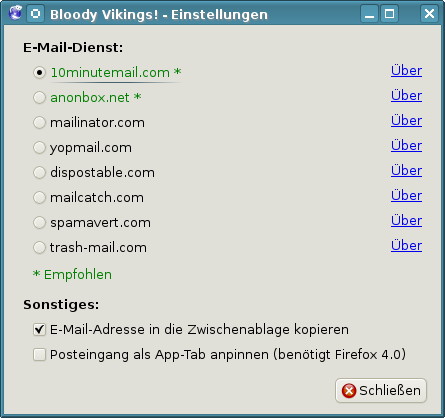
\includegraphics[scale=0.75]{../screenshots/bloody-vikings.png}
\caption{Bloody Vikings konfigurieren}
\label{abb:bloodyvikings}
\end{center}
\end{figure}

In Zukunft kann man in jedem Anmeldeformular mit der rechten Maustaste auf das Eingabefeld der E-Mail Adresse klicken und aus dem Kontextmen� den Punkt \textit{Bloody Vikings} w�hlen. Es wird in einem neuen Browser Tab die Webseite des Anbieters ge�ffnet und die tempor�re E-Mail Adresse in das Formularfeld eingetragen. Nach dem Absenden des Anmeldeformular wechselt man in den neu ge�ffneten Browser Tab und wartet auf die Best�tigungsmail.

\subsection{Private Note}
E-Mails werden auf dem Weg durch das Netz an vielen Stellen mitgelesen und ausgewertet. Ein Postgeheimnis existiert praktisch nicht. Kommerzielle Datensammler wie Google und Yahoo scannen alle Mails, die sie in die Finger bekommen. Geheimdienste wie NSA, SSSI, FRA oder BND haben Monitoringprogramme f�r den E-Mail Verkehr.\\

Gelegentlich m�chte man aber nicht, das eine vertrauliche Nachricht von Dritten gelesen wird. Verschl�sselung w�re eine naheliegende L�sung. Das ist aber nur m�glich, wenn Absender und Empf�nger �ber die n�tige Kompetenz verf�gen.\\

Als Alternative kann man folgende Dienste der Firma\textit{ insophia} nutzen:
\begin{itemize}
 \item \textit{Certified Privnote}\footnote{ \href{https://certified.privnote.com/}{https://certified.privnote.com}} ist vom ULD mit dem EuroPrise Siegel zertifiziert. Die Zertifizierung garantiert die Respektierung der Privatsph�re der Nutzer durch den Anbieter.
 \item \textit{Privnote}\footnote{ \href{https://privnote.com/}{https://privnote.com}} ist eine nicht-zertifizierten Version. Damit sind �nderungen an der Software und Weiterentwicklungen m�glich.
\end{itemize}

Man schreibt die Nachricht auf der Webseite des Anbieters und klickt auf den Button \textit{Create Note}. Javascript muss daf�r freigegeben werden. Es wird ein Link generiert, unter dem man die Nachricht EINMALIG abrufen kann. Die Daten werden verschl�sselt auf dem Server gespeichert und nur der Link enth�lt den Key, um die Daten zu entschl�sseln.\\

Den Link sendet man per E-Mail dem Empf�nger der Nachricht. Er kann die Nachricht im Browser abrufen. Nach dem Abruf der Nachricht wird sie auf dem Server gel�scht, sie ist also nur EINMALIG lesbar. Darauf sollte man den Empf�nger hinweisen.\\

Man kann den Link NICHT �ber irgendwelche Kan�le in Social Networks (z.B. Facebook) versenden. Wenn man auf den Link klickt, l�uft im Hintergrund ein Crawl der Seite bevor man weitergeleitet wird. Facebook holt sich die Nachricht und der Empf�nger kommt zu sp�t.\\

\textit{PrivNote} ist nicht kryptografisch abh�sicher wie die E-Mail Verschl�sselung mit OpenPGP. Wenn ein Angreifer unbedingt den Inhalt der Nachricht lesen will, kann er die Nachricht vor dem Empf�nger abrufen und �ber den Inhalt Kenntnis erlangen. Der eigentliche Empf�nger kann nur den Angriff erkennen, da die Nachricht auf dem Server gel�scht wurde. Damit sind die Angebote f�r private Nachrichten geeignet, aber nicht geeignet f�r geheime oder streng vertrauliche Informationen.\\

Es gibt einige �hnliche Projekte, die ich NICHT empfehle: 
\begin{itemize}
 \item \textit{Burn Note} erfordert eine Registrierung mit E-Mail Adresse, was �berfl�ssig ist. F�r jeden Account wird die Nutzung des Dienstes protokolliert und eine monatliche Statistik erstellt. Au�erdem werden die Notes mit einem Key verschl�sselt, der auf dem Server von Burn Note gespeichert wird. Im Gegensatz zu den Privnote-Diensten von insophia ist der Betreiber damit in der Lage, die Nachrichten zu entschl�sseln.

 \item Road-Message sammelt aus meiner Sicht zuviel Daten. Beim Besuch der Webseite wird besipielsweise die innere Gr��e des Browserfensters ausgelesen, was ein sehr individueller Wert ist und gut f�r das Tracking nutzbar. Es gibt keine Privacy Policy auf der Webseite, welche Daten gespeichert werden und wie die Daten genutzt werden. Auch bei Road-Message wird der Schl�ssel f�r das Entschl�sseln der Nachricht nicht in der URL kodiert (wie bei den Diensten von \textit{insophia}) sondern auf dem Server gespeichert.
\end{itemize}

\subsection{RSS-Feeds}
RSS-Feeds bieten die M�glichkeiten, sich schnell �ber Neuigkeiten in h�ufig gelesenen Blogs zu informieren ohne die Webseiten einzeln abklappern zu m�ssen. Thunderbird enth�lt einen RSS-Reader, den man daf�r nutzen kann.\\

Um mehrere interessante RSS-Feeds zu sammeln, erstellt man in der \textit{Konten Verwaltung} ein neues Konto und w�hlt den Typ \textit{Anderes Konto hinzuf�gen...}.
\begin{center}
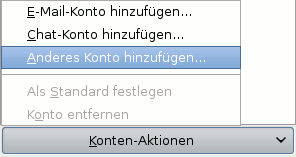
\includegraphics[scale=0.75]{../screenshots/thunderbird-rss0.png}
\end{center}

Im zweiten Schritt w�hlt man den Typ \textit{Blogs und RSS-Feeds} und danach eine beliebige Konten�bezeichnung.\\

In den Einstellungen f�r das RSS-Feed Konto kann man festlegen, in welchem Intervall die Feeds abgerufen werden sollen und ob die RSS-Feeds beim Start von Thunderbird aktualisiert werden sollen. Danach kann man die \textit{Abonnements verwalten} und die Adressen der RSS-Feeds hinzuf�gen. Man kopiert die URL des RSS-Feeds von der Webseite des Blogs in das Feld f�r die Feed URL und klickt auf den Button \textit{Hinzuf�gen} wie im Bild \ref{abb:addrssfeeds} dargestellt.\\
\begin{figure}[htb]
\begin{center}
 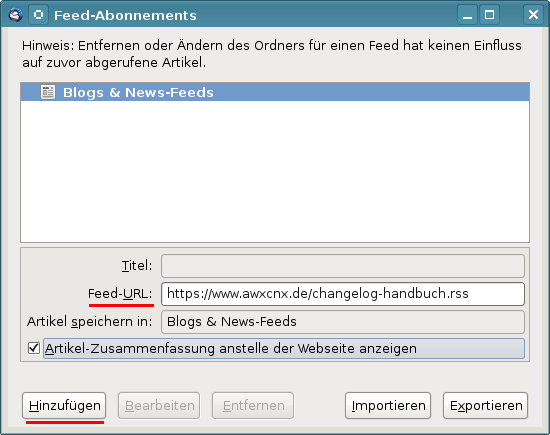
\includegraphics[scale=0.75]{../screenshots/thunderbird-rss2.png}
\caption{RSS-Feed hinzuf�gen}
\label{abb:addrssfeeds}
\end{center}
\end{figure}

Die Neuigkeiten aus den Blogs kann man zuk�nftig wie E-Mails lesen. Dabei kann man eine simple Textanzeige w�hlen oder die Ansicht als Webseite. Wer die Ansicht als Webseite bevorzugt, sollte Javascript, Cookies und andere Tracking Elemente deaktivieren. Zum Kommentieren muss man allerdings die Webseite des Blogs im Browser aufrufen.

\subsection{Filelink}
Seit Version 13.0 bietet Thunderbird die M�glichkeit, gro�e Dateianh�nge bei einem Filehoster hochzuladen und dem Empf�nger nur den Link zum Download per E-Mail zu senden. In der Version 16.0 unterst�tzt Thunderbird die Filehoster YouSendIt\footnote{ \href{https://www.yousendit.com}{https://www.yousendit.com}} und Box.net\footnote{ \href{https://www.box.com/}{https://www.box.com/}} sowie Ubuntu One.\\

Ich kann dieses Feature nicht empfehlen. 
\begin{enumerate}
 \item YouSendIt protokolliert alle Aktivit�ten und die Protokolle werden f�r drei Jahre gespeichert: 
 \begin{quote}
  \textit{YouSendIt will retain the Log Data collected from you in its active, internal company databases for up to six months, at which point it will migrate such Log Data to its offline archival systems, where YouSendIt will retain the Log Data for a period of three years.}
 \end{quote} 
 \item Die bei einem Cloud-Service gespeicherten Dateianh�nge unterliegen nicht dem besonderen Schutz des Post- und Fernmeldegeheimnisses.
 \item Au�erdem ist das Filelink nicht in die E-Mail Verschl�sselung integriert. Auch wenn man eine verschl�sselte E-Mail schreibt, werden die Uploads unverschl�sselt auf dem Server abgelegt. Man muss sich selbst um die Verschl�sselung der Dateien k�mmern. Dann kann man sie auch gleich selbst zu einem 1-Click-Hoster hochladen.
\end{enumerate}

Um nicht st�ndig mit der Frage bel�stigt zu werden, ob man einen gro�en Dateianhang bei einem Cloude-Anbieter speichern m�chte, kann man das Feature in den Einstellungen deaktivieren. 
\begin{figure}[htb]
\begin{center}
 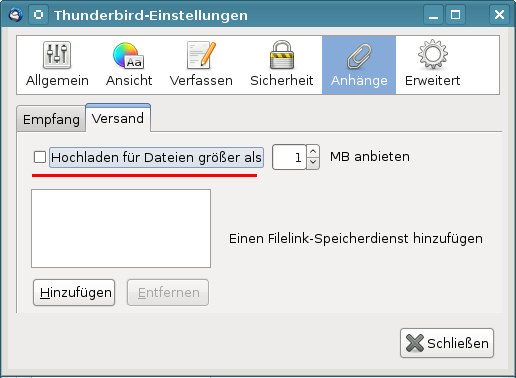
\includegraphics[scale=0.75]{../screenshots/tb-filelink.png}
\caption{Filelink deaktivieren}
\label{abb:filelink}
\end{center}
\end{figure}

\end{document}